\chapter{Literature Survey} \label{ch2}
In this chapter a brief discussion of work done by various researchers in this area for the last two decades is presented. Balaji and Venkateshan\citep{BALAJI1993260} have developed a model to investigate the significance of radiation in natural convection inside a square cavity. Even though their work does not discuss solar applications, it has shown light to heat loss mechanisms that are taking place in a cavity. Work of Balaji and Venkateshan [12] can be considered as the first proper attempt to prove the effect of radiation in free convection cavity problems. For convection, Boussinesq approximation has been used for simplification of the governing equations. They have developed a correlation to obtain radiation and convection Nusselt number. They have also shed light on "dual nature" of radiation. The increase in radiation causes convection Nusselt number to drop while overall Nusselt number which is the combination of both radiation and convection Nusselt numbers can either increase or decrease depending on other factors like emissivity of walls, temperature ratio etc. Pye et. al.\cite{pye2003modelling} modeled a simple trapezoidal cavity with emissivity and temperature values close to the actual values of the experiment. They assumed a constant temperature for the absorber. The simulation was done in Fluent 6.0 for different cavity depth, cavity width, the temperature of absorber plate, ambient temperature and convection coefficient of outer surface the glass covering. For convection, Boussinesq approximation is used and Discrete Transfer Model for radiation (DTRM) is used. Grid size used was $2\ mm$ where triangular grids used in the side walls and rest square grids are used. They have depicted heat flow process from absorber as described further. Absorber receives solar radiation and its temperature rises. Other surfaces of cavity receive heat from absorber through a combination of conduction, convection and radiation. Heat energy then gets conducted to external surfaces of the cavity receiver. Then through a combine effect of convection and radiation, it escapes the cavity. Radiation dominates the internal heat transfer process because absorber temperature is very high and heat transfer through radiation is proportional to differences in the fourth power of surface temperatures. Convection contributes only 8\% of total heat transfer inside the cavity. Convection dominates in heat transfer exchange between the outer surface of the cavity and surroundings. Because the glass, through which heat is mainly transferred to the atmosphere; is not at that high temperature from the outside air They also found that the top space of the cavity is almost stratified so that only conduction is present and at the bottom part convection is present at very
low velocity which explains the low convection percentage in the losses. They proposed relations for external as well as internal radiation and convection losses. They fixed all non-dimensional parameters like emissivity and external heat transfer coefficient and varied only depth and width of the cavity. Other non-dimensional parameters are found for the air temperature inside the cavity (approximated by taking an average of glass cover temperature and
absorber tube temperature. The relation given by them for the convective Nusselt number inside the cavity is as follows.
\begin{equation}
Nu_{conv} = 1.1917(Gr)^{.10363}(D/W)^{.6432}
\end{equation}
For internal radiation losses, they proposed simple parallel plate formula and for external
radiation and convection losses; normal convection radiation formulas for a plate at constant
temperature is proposed.

Singh et. al.\citep{SINGH2010329} introduced different shapes and coatings for the absorber. Their studies were completely experimental. They used a single square shaped absorber as well as six round absorber pipes in the trapezoidal cavity. They combined normal coating and selective coating in them and studied the changes in thermal performance. They also introduced a double glass cover since most of the losses are occurring through the glass cover. They passed oil through the absorber and found out the heat loss from entry to exit and equated it to the heat loss taking place from the absorber to the other components, thus obtained the heat transfer coefficient. They also the selective coating offered 20-30\% less heat transfer coefficient compared to the ordinary black paint. The use of double glass covers of the cavity offered a 10-15\% lower heat transfer coefficients for different absorber temperature. They developed a correlation between heat transfer coefficient and absorber temperature. They also found out the values analytically by using correlation obtained by Balaji and Venkateshan\citep{BALAJI1994249} and correlation for heat transfer coefficient between parallel plates.
However, both showed a significant difference from the experimental values.
All of these CFD models were able to show the flow patterns correctly. However, the losses predicted showed a significant variation. Reynolds et. al.\citep{REYNOLDS2004229} predictions using CFD model showed excellent agreement with actual flow pattern. They compared their simulation result using Fluent 5.0 with the experimental results. They observed the same pattern in the simulated model and experimental model which can be seen in fig.\ref{rey}. 

\begin{figure}[H]
\begin{center}
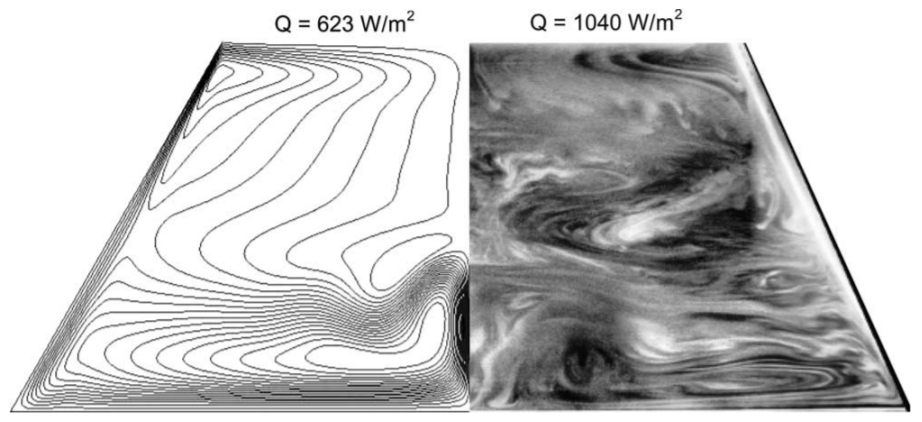
\includegraphics[width=\textwidth]{reynolds40.PNG}
\caption{Comparison between CFD simulated from pattern
(left) to the experimentally observed pattern obtained by
Reynolds et. al.\citep{REYNOLDS2004229}}
\label{rey}
\end{center}
\end{figure}

They also observed that the 2/3rd of the cavity in the top is thermally stratified and the remaining part of the cavity has counter-rotating flows on either side of the symmetry plane. Even though their flow pattern is in excellent agreement with the CFD simulated model, the CFD model under predicted the losses by more than 40\%. Their explanation was that it is because of the uncertainties in measurement. At this point Fac\~ao and Oliveira\citep{FACAO201190} used a new model where the absorber is modeled as a lower half of the pipes with no gap as shown in the Fig.\ref{facao}

\begin{figure}[H]
\begin{center}
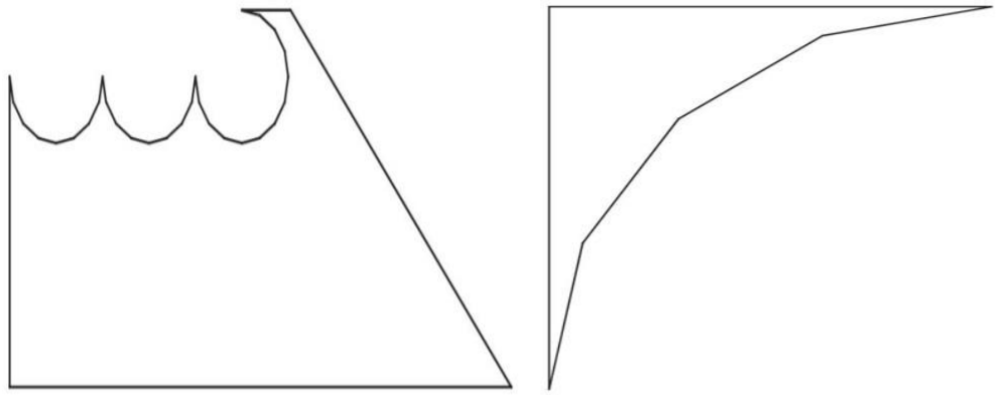
\includegraphics[width =\textwidth]{faco.PNG}
\caption{Modified model of trapezoidal cavity including the pipes (left) Circular cross-section of pipe approximated
as hexadecagons for easy meshing and faster convergence (Right) proposed by Pye et. al.\citep{pye2003modelling}}
\label{facao}
\end{center}
\end{figure}

Initially, this model is proposed by Pye in his Ph.D. thesis\citep{pye2008system}. Pye et. al.\citep{pye2003modelling} simulated heat losses in the cavity using Fluent and found that radiation losses are 25\% higher than the value obtained when an isothermal flat surface is used. Therefore, they concluded that geometry of the pipe does matter in heat loss analysis. Fac\~ao and Oliveira\citep{FACAO201190} took this observation and approximated lower half circle as regular hexadecagons as shown in Fig.\ref{facao} to avoid convergence issues and inaccuracies. They changed two geometric parameters which are the depth of the cavity and insulation thickness of sidewall. Also, they considered two different heat transfer coefficients for the external side of the glass cover to accommodate two different wind velocities. Total eighteen sets of simulations are carried out using combinations of these parameters. They compared the heat transfer coefficients obtained with the other available literature and found that their values are significantly higher; that means closer to the experimental values and hence showed the importance of inclusion of geometry of the pipes. Different values thickness of insulation and depth of cavity were used in their simulation to find out heat transfer coefficient and choose the best thickness and depth by trial and error. Flow pattern obtained by him for the modified geometry is shown in Fig.\ref{facaoresult}

\begin{figure}[H]
\begin{center}
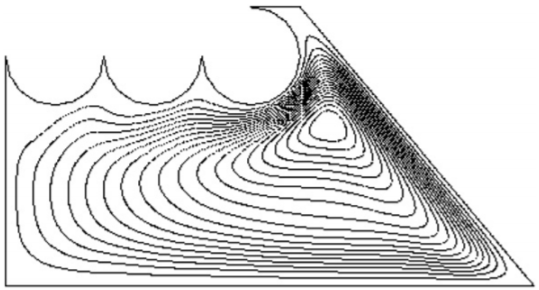
\includegraphics[width=\textwidth]{facoresult.PNG}
\caption{ Stream lines obtained in model with modified geometry by Fac\~ao and Oliveira\citep{FACAO201190}}
\end{center}
\label{facaoresult}
\end{figure}


Later, Sahoo et. al.\citep{SAHOO201318} modeled full absorber pipes of certain numbers with gaps between them. They validated their result with experimental models and then analyzed the effect of various parameters such as receiver tube surface temperature, receiver depth, the number of tubes, and emissivity of the outer surface of the receiver tubes. They have concluded that contribution of convection is between 5\% and 18\% of the total heat losses. They got an excellent agreement between the simulated results and the experimental heat transfer values except at high temperatures. Their explanation was that it is because of the approximation that top of the cavity is completely insulated and heat loss from it was neglected. They compared the obtained heat transfer coefficient values with the results by Fac\~ao and Oliveira\citep{FACAO201190} and Pye et. al.\citep{pye2003modelling}. They got an increase of 24-29\% increase with respect to Pye et. al.\textquotesingle s values and 4-13\% increase with respect to Fac\~ao and Oliveira\textquotesingle s values. The obtained temperature contour is shown in fig.\ref{sahooresult}

\begin{figure}[H]
\begin{center}
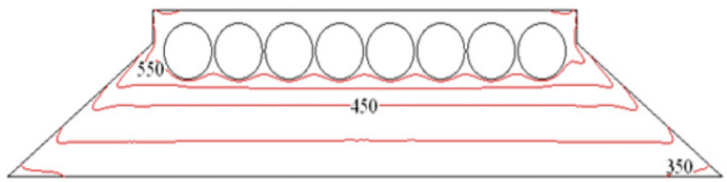
\includegraphics[width=\textwidth]{sahooresult.PNG}
\caption{Isotherms obtained by Sahoo et. al. for 8 pipes with gap\citep{SAHOO201318}}
\end{center}
\label{sahooresult}
\end{figure}

Natarajan et. al.\citep{NATARAJAN2012523} again assumed the flat absorber top for their CFD simulations but did not use Boussinesq approximation. They have solved 2-D geometry with laminar and steady-state condition using implicit solver. For changes in viscosity, it calculated by using Sutherland\textquotesingle s theory of viscosity with three coefficient method. They made a point that Boussinesq approximation is not valid for temperature above $100^0\ C$ which is the case at the top part of the cavity. They studied heat losses by varying aspect ratio, temperature ratio, Grashof number, surface emissivity, absorber angle and radiation conduction number. As per their observation, increasing the aspect ratio causes increment in the thickness of the static air region near the upper part of the cavity which reduces the overall loss of heat in a trapezoidal cavity. The increment in temperature ratio causes increased difference in temperature between the top wall and the bottom wall of the cavity but has negligible effect on the thickness of static air zone. However, it reduces heat transaction between top and bottom wall but this decrement becomes sluggish beyond certain temperature ratio($T_c/T_h$) equal to $0.6$. Thus, in general, heat loss in a trapezoidal cavity can be reduce to a certain extent by increasing aspect ratio and temperature ratio. Moghimi et. al.\citep{MOGHIMI2015343} modeled a full cavity with insulations and used CFD tools to optimize the cavity design to minimize the losses as well as to get desired wind resistance. They have used discreet ordinate (DO) method to include the semi-transparent properties of glass. From the
temperature patterns they have observed that below the pipes; radiation and conduction heat transfer dominates as can be seen from fig.\ref{optz}.

\begin{figure}[H]
\begin{center}
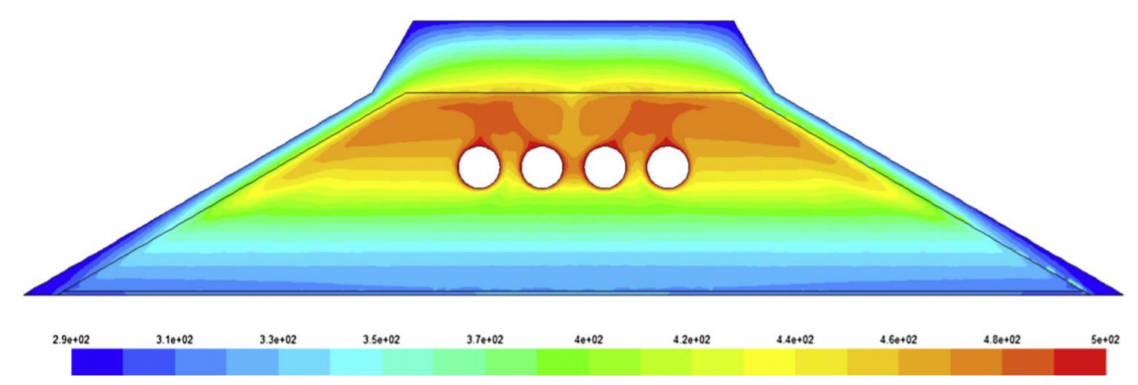
\includegraphics[width=\textwidth]{optz.PNG}
\caption{Temperature contour obtained by Moghimi et. al.\citep{MOGHIMI2015343}}
\end{center}
\label{optz}
\end{figure}

All the research work until this point have been done by solving Navier-Stokes equation for convection. But convection consists of two heat transfer methods namely conduction and advection. Mohan et.al. \citep{MOHAN201837} have shown that conduction accounts for more than 99\% of heat transfer by convection. To prove this they have shown two studies on trapezoidal cavity receiver. First study shows comparison of heat transfer using convection against heat transfer using conduction only in TCR. Obtained results show remarkable similarity. Second study shows comparison of heat transfer using convection+radiation against heat transfer using conduction+radiation. Again in this study results obtained from both the methods are quite close. Obtained Nusselt number at the hot in both the cases is within 1\% of each other which can be seen in the following table \ref{tab:sarathcomptable}. This study shows that even if we take conduction and radiation as heat transfer method in a TCR, same results can be achieved as with convection and radiation as extent of advection is quite insignificant. This also gives an advantage by reducing complexity of the model as Navier-Stokes equation has no longer to be solved.

\begin{table}[H]
\centering
\caption{Heat flux and Nusselt number of hot wall in a trapezoidal cavity}
\label{tab:sarathcomptable}
\begin{tabular}{|c|c|c|l|l|}
\hline
\textit{\textbf{At the hot wall}} & \textbf{Convection} & \textbf{Conduction} & \textbf{\begin{tabular}[c]{@{}l@{}}Convection+\\ Radiation\end{tabular}} & \textbf{\begin{tabular}[c]{@{}l@{}}conduction+\\ Radiation\end{tabular}} \\ \hline
Total heat (W)                    & 50.06               & 49.00               & 899.90                        & 892.27                        \\ \hline
Total radiation heat (W)          & 0.00                   & 0.00                   & 845.96                        & 846.99                        \\ \hline
Nusselt number                    & 1.12                & 1.10                & 20.24                         & 20.07                         \\ \hline
\end{tabular}
\end{table}













